\documentclass{article}
\usepackage{geometry}
\usepackage{graphicx}
\geometry{   rmargin=1in
            ,lmargin=1in
            ,tmargin=1in
            ,bmargin=1in
         }

\begin{document}

\begin{flushright}
   Context-Free
\\ Prof. Omer Soysal
\\ CSC 7700-004
\\ \today 
\end{flushright}

\section{Requirements}
\begin{itemize}
 \item \textbf{Primary goal}: to minimize the likelihood of pedestrian and driver casualties due to inaccuracies and inefficiencies in sign, crosswalk, and pedestrian detection algorithms.
 \item \textbf{Secondary goals, objectives, and tasks}: 
  \begin{enumerate} 
    \item \textbf{Goal}: stop sign detection. Detect stop signs in real-time with sufficient efficiency to allow for stopping time. Test SURF against two alternate algorihtms, described below.
    \begin{enumerate} 
     \item \textbf{Objective}: construct and R-channel integral-image-based detector.
      \begin{enumerate}
       \item \textbf{Task}: compute integral image on the R-channel of the image. 
       \item \textbf{Task}: superimpose an $m$x$m$ grid on the image and compute the
                   sums of the R-channel intensity per $2$x$2$ region.
       \item \textbf{Task}: for the $2$x$2$ region with the maximum sum, recursively
                   apply (ii) until the region with the maximum R-channel
                   intensity density  is obtained.
       \item \textbf{Task}: in the neighboorhoods of the vertices inside the
                   maximum-density region, find the four box such that the
                   diagonal along those boxes separates a maximum-density
                   R-channel triangle from a minimum-density R-channel
                   triangle.
       \item \textbf{Task}: obtain the 8 vertices of the sign from the above.
      \end{enumerate} 
     \item \textbf{Objective}: construct octagon detector.
      \begin{itemize} 
       \item \textbf{Task}: apply a shape detector to yield sets of vertices.
       \item \textbf{Task}: discard all sets where $n \neq 8$.
       \item \textbf{Task}: check to see if the opposing edges of the 8-vertex
                   shape are parallel (within a certain threshold).
      \end{itemize} 
    \end{enumerate} 
    \item \textbf{Goal}: pedestrian crosswalk sign detection.
     \begin{enumerate} 
     \item \textbf{Objective}: construct and RG-channel integral-image-based detector.
      \begin{enumerate}
       \item \textbf{Task}: compute integral image on the R-channel of the image. 
       \item \textbf{Task}: superimpose an $m$x$m$ grid on the image and compute the
                   sums of the R-channel intensity per $2$x$2$ region.
       \item \textbf{Task}: for the $2$x$2$ region with the maximum sum, recursively
                   apply (ii) until the region with the maximum R-channel
                   intensity density  is obtained.
       \item \textbf{Task}: in the neighboorhoods of the vertices inside the
                   maximum-density region, find the two boxes such that the
                   diagonal along those boxes seperates a maximum-density
                   RG-channel triangle from a minimum-density RG-channel
                   triangle.
       \item \textbf{Task}: obtain the 3 vertices of the sign from the above.
      \end{enumerate} 
    \end{enumerate} 
  \end{enumerate} 
\end{itemize}

\section{Design}
\begin{itemize}
 \item \textbf{Modules}
 \begin{enumerate} 
  \item \textbf{SignDetector1}:
   \begin{itemize} 
    \item \textbf{Functionalities}: computes and uses integral image on the R-channel
          to find maxmium-density areas used to approximate the region occupied
          by the stop sign. 
    \item \textbf{Data structures}: 
     \begin{itemize}
      \item \textbf{Namespaces}: \texttt{EmguCV.CV}.
      \item \textbf{Classes} (\texttt{Image}) and \textbf{class members}:
        \texttt{Resize()},       \texttt{Convert()},
     \end{itemize}
   \end{itemize} 
  \item \textbf{SignDetector2}:
   \begin{itemize} 
    \item \textbf{Functionalities}: uses edge detection, then isolates eight vertices
          with maximum octagonality.
    \item \textbf{Data structures}: 
          \texttt{Image, LineSegment2D, boxList, triangleList, Contour}
     \begin{itemize}
      \item \textbf{Namespaces}: \texttt{EmguCV.CV}.
      \item \textbf{Classes} (\texttt{Image}, \texttt{Contour}) and \textbf{class members}:
        \texttt{Canny()},        \texttt{HoughLinesBinary()},
        \texttt{Resize()},       \texttt{Convert()},
        \texttt{PyrUp()},        \texttt{PyrDown()},
        \texttt{FindContours()}.
     \end{itemize}
   \end{itemize} 

  \item \textbf{PedDetector}:
   \begin{itemize} 
    \item \textbf{Functionalities}: detects pedestrians using built-in EmguCV classes.
    \item \textbf{Data structures}: \texttt{Rectangle[]}.
     \begin{itemize}
      \item \textbf{Namespaces}: \texttt{EmguCV.CV}.
      \item \textbf{Classes} (\texttt{Image}, \texttt{HOGDescriptor}) and \textbf{class members}: 
       \texttt{Draw()},
       \texttt{SetSVMDetector()},
       \texttt{DetectMultiScale()},
       \texttt{GetDefaultPeopleDetector()}.
     \end{itemize}
   \end{itemize} 

%  \item LaneMarkingDetector: \ldots
%   \begin{itemize} 
%    \item \textbf{Functionalities}: \ldots
%    \item \textbf{Data structures}: \ldots
%     \begin{itemize}
%      \item \textbf{Namespaces}: \ldots
%      \item \textbf{Classes} and \textbf{class members}: \ldots
%     \end{itemize}
%   \end{itemize} 

 \end{enumerate} 
\end{itemize} 

\pagebreak

\begin{center}
 \begin{figure}
  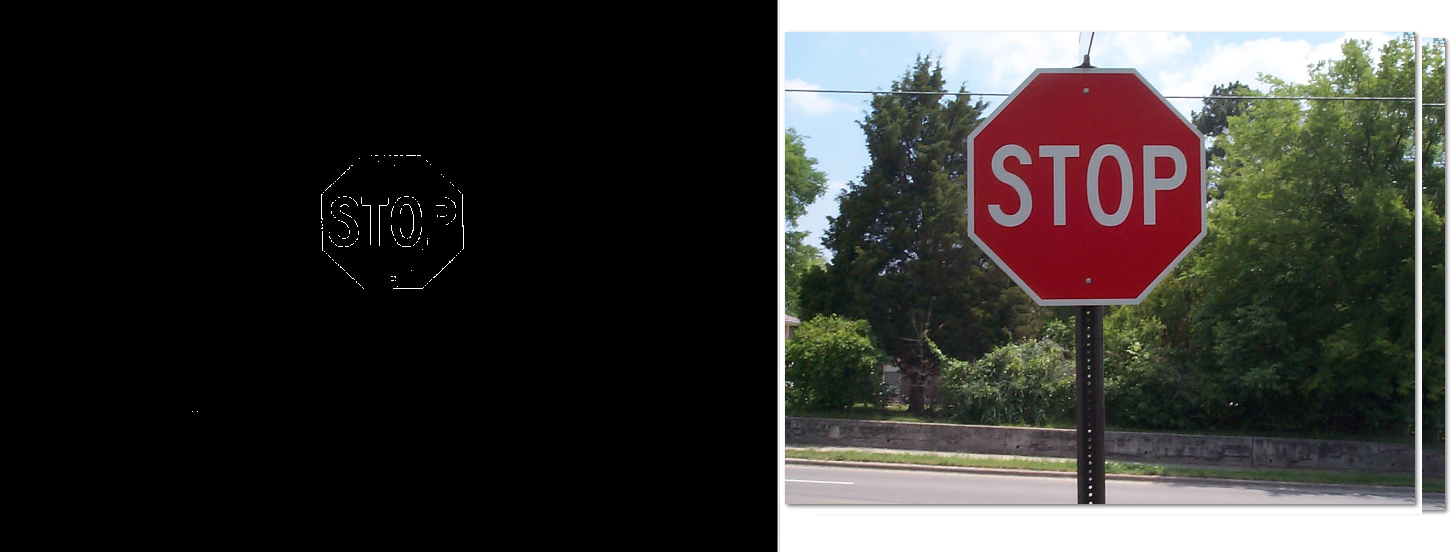
\includegraphics[width=\textwidth]{1.png}
  \caption{Edge detector by computing R-(G+B), clamped from 0 to 255}
 \end{figure}
 \begin{figure}
  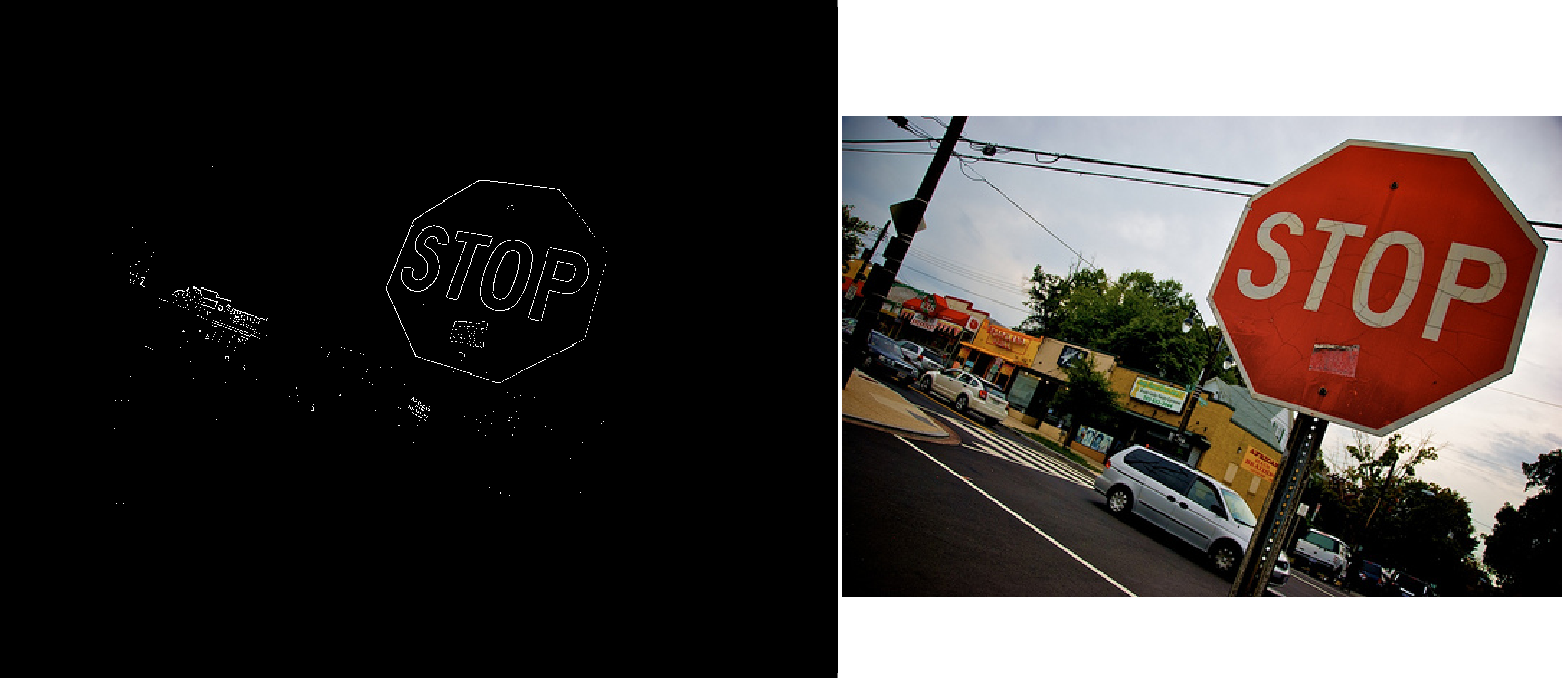
\includegraphics[width=\textwidth]{3.png}
  \caption{Edge detector by computing R-(G+B), clamped from 0 to 255}
 \end{figure}
\end{center}

\end{document}
